\en

\section{Refactoring}

Martin Fowler defines refactoring as ``a controlled technique for improving the design
of an existing code base. Its essence is applying a series of small
behavior-preserving transformations, each of which is too small to be worth
doing. However, the cumulative effect of each of these transformations is quite
significant''~\citep{refactorbook}. Eliminating detected code clones and
duplication is a refactoring task that requires the application of refactoring
methods. Fowler presents several refactoring techniques, including
\textit{parameterize method}, \textit{replace parameter with explicit methods},
and \textit{replace parameter with method}~\citep{refactorbook}. Below is a
brief explanation of the methods used in our research.

\begin{figure}[ht]
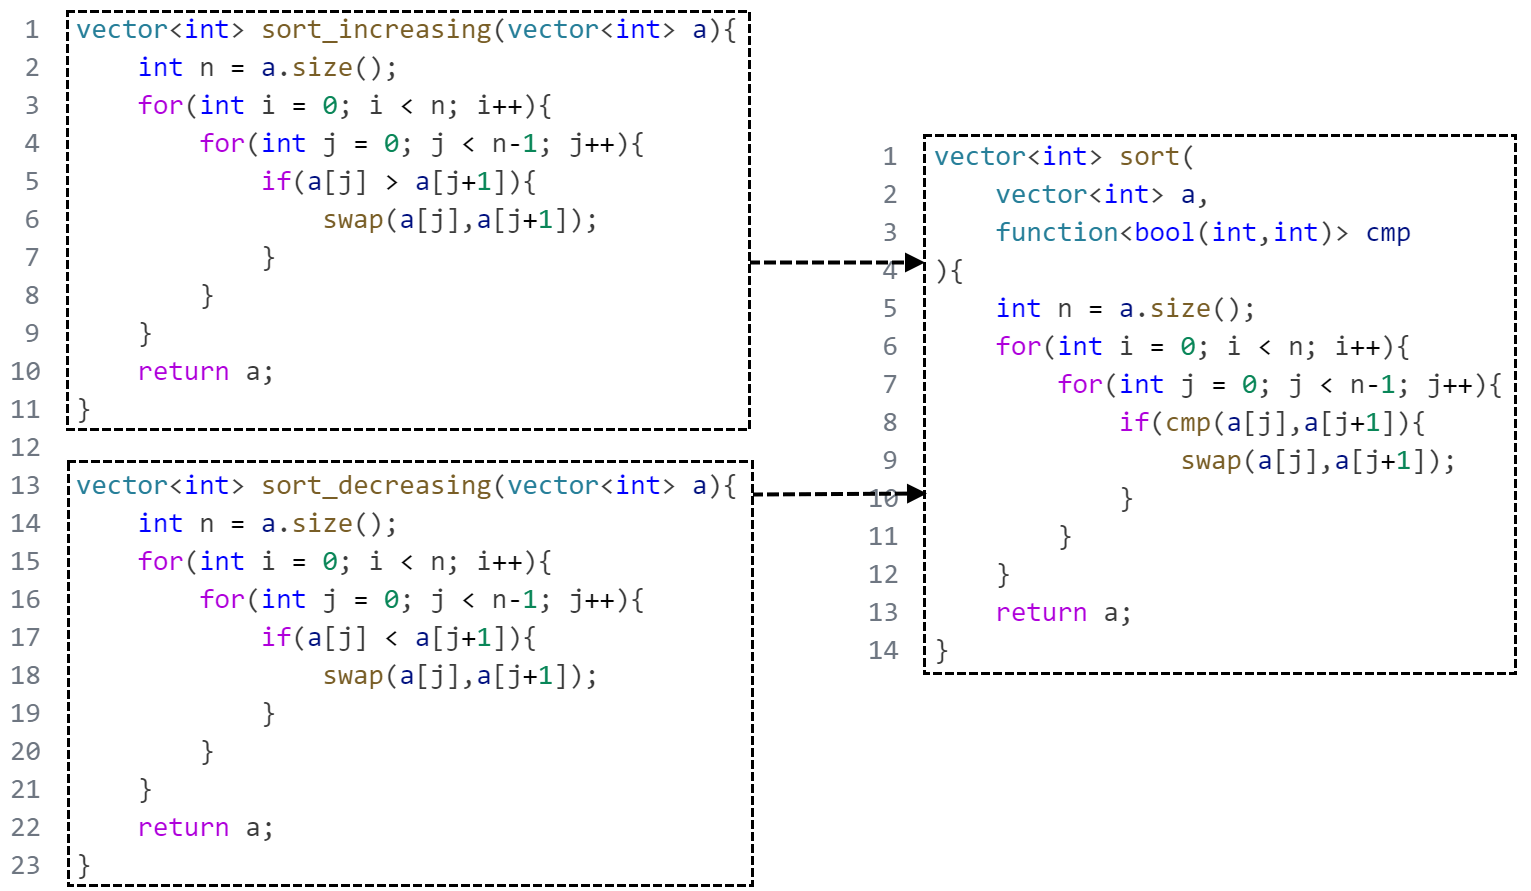
\includegraphics[scale=0.36]{refactor/parameterize}
\caption{Example of Parameterize Method usage.}
\label{fig:parameter}
\end{figure}

\paragraph{Parameterize Method.}
The Parameterize Method involves replacing multiple similar code blocks with a
single function. This function incorporates parameters to account for the
different behaviors across similar code snippets, allowing it to adjust
functionality based on the parameter values~\citep{refactorbook}.
Figure~\ref{fig:parameter} illustrates an example of the Parameterize Method.


\begin{figure}[ht]
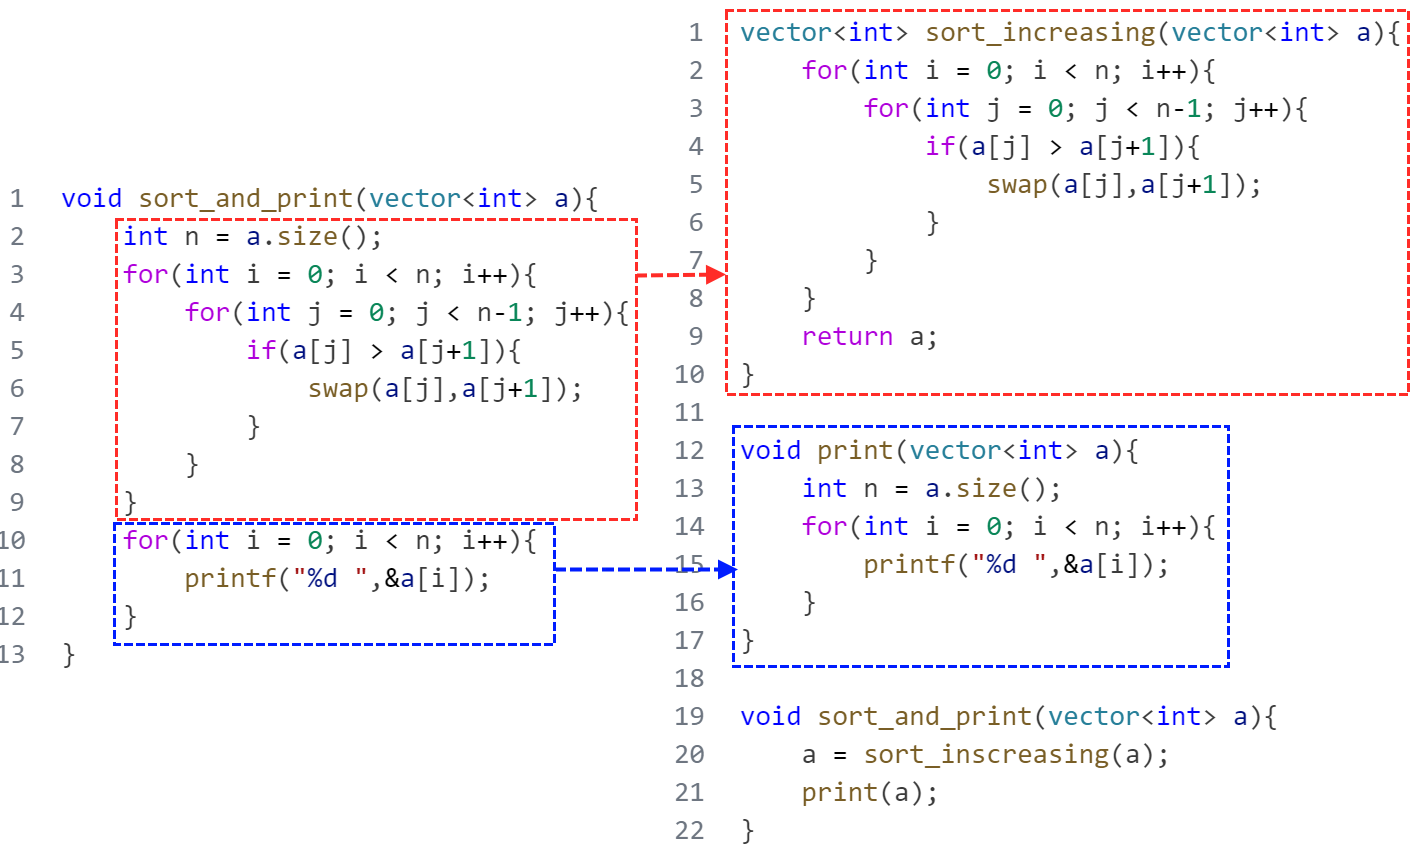
\includegraphics[scale=0.36]{refactor/extract}
\caption{Example of Extract Method usage.}
\label{fig:extract}
\end{figure}


\paragraph{Extract Method.}
The Extract Method entails breaking down a complex code artifact into multiple,
simpler methods or functions. One of the primary advantages of this method is
that the newly created functions can be reused throughout the project. By
contrast, a complex code artifact might not be entirely reusable, potentially
resulting in further code duplication~\citep{refactorbook}.
Figure~\ref{fig:extract} demonstrates an example of the Extract Method.

\paragraph{Inline Method.}

The inline method involves replacing a function call with the entire body of 
the function, which is copied to where the function is called. One of the 
advantages of this method is reducing the number of unnecessary methods and 
abstraction in the code, making the code more straightforward~\citep{refactorbook}.

